\documentclass[11pt]{article}
\usepackage{amsmath,textcomp,amssymb,geometry,graphicx,hyperref,mathtools,textcomp}
\usepackage[final]{pdfpages}
\usepackage[export]{adjustbox}
\usepackage{enumerate}
\usepackage{titlesec}
\usepackage{listings}
%\usepackage[usenames, dvipsnames]{color}
\usepackage{cleveref}

\lstdefinestyle{customc}{
  belowcaptionskip=1\baselineskip,
  breaklines=true,
  frame=L,
  xleftmargin=\parindent,
  language=C,
  showstringspaces=false,
  keywordstyle=\bfseries\color{green!40!black},
  commentstyle=\itshape\color{purple!40!black},
  identifierstyle=\color{blue},
  stringstyle=\color{orange},
}

\lstset{escapechar=@,style=customc}

\def\Name{Achal Dave}
\def\CourseName{10-725}
\def\CourseSemester{Fall}
\def\CourseYear{2016}

\title{Scribe Notes: Duality in General Programs}
\author{\Name}
\markboth{\CourseName\ -- \CourseSemester\ \CourseYear\ -- Lecture}{\CourseName\ -- \CourseSemester\ \CourseYear\ -- Lecture}
\pagestyle{myheadings}

\DeclarePairedDelimiter\ceil{\lceil}{\rceil}%
\DeclarePairedDelimiter\floor{\lfloor}{\rfloor}%
\DeclarePairedDelimiter\abs{\lvert}{\rvert}%
\DeclarePairedDelimiter\norm{\lVert}{\rVert}%
\newcommand{\E}{\mathbb{E}}
\newcommand{\R}{\mathbb{R}}
\newcommand{\st}{\text{s.t.}}
\newcommand{\Var}{\mathrm{Var}}
% From http://tex.stackexchange.com/questions/79434/
\newcommand\independent{\protect\mathpalette{\protect\independenthelper}{\perp}}
\def\independenthelper#1#2{\mathrel{\rlap{$#1#2$}\mkern2mu{#1#2}}}

\begin{document}

\maketitle

\section{Last Class: Duality in Linear Programs}

In last class, we discussed two explanations for how we formulate the dual problem in linear programs.\\
\textit{Explanation \#1}: We multiply the corresponding dual variables to each of the constraints in the primal problem and sum the expressions. This gives us an expression similar to the primal criterion which is lower bounded. Equating this expression to the primal criterion, we get equality constraints, in addition to the inequality constraints obtained by introducing the dual variables. \\
\textit{Explanation \#2}: Alternatively, we can construct the Lagrangian by introducing a dual variable for each constraint, multiplying it with the constraint and adding it to the criterion. We can observe that the Lagrangian (constructed this way) is a lower bound on the primal criterion, for any value of the dual variables. This method reproduces the same dual as \#1 above, but is actually completely general and applies to arbitrary optimization problems (even non-convex programs and not just linear programs)


\section{Lagrangian}

Consider any general minimization problem
\begin{alignat*}{2}
&\min_x &&f(x) \\
&\text{ subject to}&~&h_i(x) \leq 0, i = 1, \dots, m \\
&&&l_j(x) = 0, j = 1, \dots, r
\end{alignat*}

Let's define the Lagrangian, introducing variables $u \in \R^m, v \in \R^r$,
with $u \geq 0$.
\begin{align*}
L(x, u, v) = f(x) + \sum_{i=1}^m u_i h_i(x) + \sum_{j=1}^r v_j l_j(x)
\end{align*}

It turns out that for any $u \geq 0$ and any $v$, we have that
\begin{align*}
L(x, u, v) = f(x) \sum_{i=1}^m u_i \underbrace{h_i(x)}_{\leq 0} + \sum_{j=1}^r v_j \underbrace{l_j(x)}_{=0} \leq f(x)
\end{align*}
Thus, we can observe that the Lagrangian $L(x, u, v)$ is always a lower bound for the primal criterion $f(x)$ for any value of $u \geq 0$ and $v$. An example for this is shown in the figure below:

\begin{figure}[h]
  \centering
  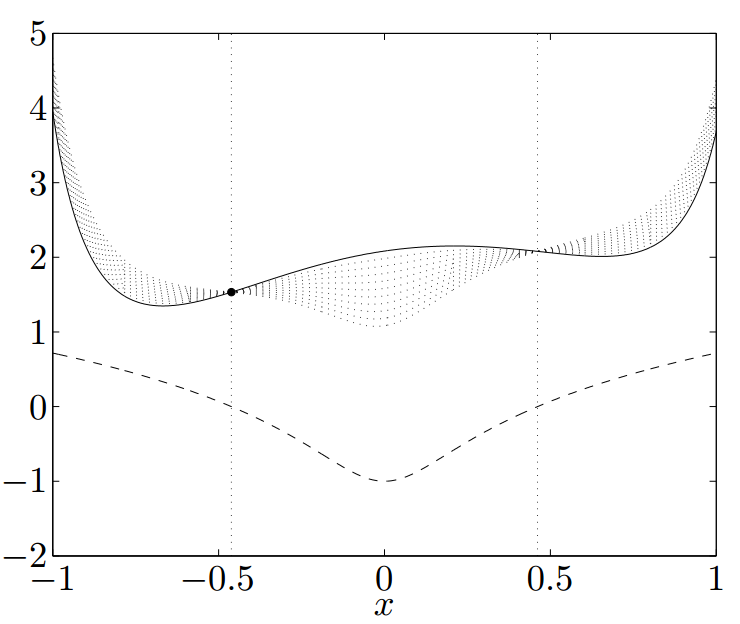
\includegraphics[scale=0.3]{lagrangian.png}
  \caption{Solid line is $f$, dashed line is $h$. Each dotted line shows $L(x,u,v)$ for different choices of $u \geq 0$ and $v$. Note that the feasible set is $x \in [-0.46, 0.46]$}
  \label{fig:lagrangian}
\end{figure}

And so, we have that if $f^*$ be the primal optimal value and $C$ is the primal
feasible set, then
\begin{align*}
f^* \geq \min_{x \in C} L(x, u, v) \geq \min_x L(x, u, v) \triangleq g(u, v)
\end{align*}

This $g(u, v)$ is the \textbf{Lagrange dual function}, and it provides a lower
bound on the optimal value $f^*$ for any dual feasible $u, v$ (i.e. $u \geq 0$
and any $v$).

Generally, duality will provide us with a tight lower bound in the
\textit{convex} case, but this need not be the true in the \textit{non-convex} case.

\subsection{Example: Quadratic Program}
Consider a quadratic program where $Q \succ 0$:
\begin{alignat*}{2}
&\min_x& &\frac{1}{2} x^T Q x + c^T x \\
&\text{ subject to}&~&Ax = b, x \geq 0
\end{alignat*}

In this case, our Lagrangian is simply
\[ L(x, u, v) = \frac{1}{2} x^T Q x + c^T x - u^T x + v^T(Ax - b) \]

To compute the dual function $g(u, v) = \min_x L(x, u, v)$, we minimize the
Lagrangian above by taking the gradient with respect to $x$ and setting it equal
to zero, and we get that
\begin{align*}
x^* &= -Q^{-1}(c - u + A^T v) \\
\implies \min_x L(x, u, v) &= L(x^*, u, v) \\
    &= \frac{1}{2} (c - u + A^T v)^T Q^{-1}(c - u + A^T v) - (c - u + A^T v)^T Q^{-1}(c - u + A^T v) - b^T v \\
    &= -\frac{1}{2} (c - u + A^T v)^T Q^{-1}(c - u + A^T v) - b^T v
\end{align*}

What if, instead, we had the same QP as above, except $Q
\mathbin{\textcolor{red}{\succeq}} 0$ (i.e. Q is only positive
\textit{semi}-definite).  Then, if we try to minimize the Lagrangian above by
setting the gradient to 0, we get the following constraint at the optimum:
\begin{align}
Qx = -(c - u + A^T v) \label{eq:qp_semidefinite_zero_gradient}
\end{align}

Now, there are two cases:
\begin{enumerate}[(i)]
\item $c - u + A^T v \in \text{col}(Q)$. Then, we can use the pseudo-inverse (see below)
      $Q^{\dagger}$ of $Q$. This also implies that $P \left( c - u + A^T v \right) = 0$, where $P$ is the projection matrix onto $\text{null}\left(Q\right)$.
\item $c - u + A^T v \not\in \text{col}(Q)$, which implies that $c - u + A^T v$
      is not orthogonal to the null space of $Q$. Then, let
      \[ c - u + A^T v = z_1 + z_2, \]
      where $z_1 \in \text{col}(Q), z_2 \in \text{null}(Q), z_2 \neq 0$. But
      in this case, there is no $x$ that satisfies
      \cref{eq:qp_semidefinite_zero_gradient}, and so there is no unique
      minimizer $x^*$. But $L(x, u, v)$ is quadratic in $x$, so if there is no
      minimizer of $L(x, u, v)$ in $x$, the minimum must be $L(x, u, v) =
      -\infty$.
\end{enumerate}

So,
\begin{align*}
g(u, v) = \begin{cases}
-\frac{1}{2} (c - u + A^T v)^T Q^{\dagger} (c - u + A^Tv) - b^T v ~&\text{case (i)} \\
-\infty ~&\text{case (ii)}
\end{cases}
\end{align*}

\subsubsection{Aside: Pseudo-inverse}
For a general matrix $A \in \R^{n\times n}$, we can define the pseudo-inverse
$A^{\dagger}$ in terms of its Singular Vector Decomposition. Using SVD, we can
write $A$ as
\[ A = U D V^T \]

If $A$ was invertible, we can directly invert the decomposition above:
\[ A^{-1} = (U D V^T)^{-1} = (V^T)^{-1} D^{-1} U^{-1} = V D^{-1} U^T \]
where
\begin{align*}
D^{-1} = \begin{bmatrix}
\frac{1}{d_1} & 0 & \dots & 0 \\
0 & \frac{1}{d_2} & \dots & 0 \\
0 & 0 & \ddots & \vdots \\
0 & 0 & \dots & \frac{1}{d_n} \\
\end{bmatrix}
\end{align*}

If $A$ is not invertible, we're going to see that for $k = \text{rank}(A)$,
$d_{k+1} = d_{k+2} = \dots = d_n = 0$. In this case, we can construct $D^{-1}$ as follows:
\begin{align*}
D^{-1} = \begin{bmatrix}
\frac{1}{d_1} & 0 & \dots & 0 & 0\\
0 & \frac{1}{d_2} & \dots & 0 & 0\\
0 & 0 & \ddots & \vdots & 0 &\\
0 & 0 & \dots & \frac{1}{d_k} & 0 \\
0 & 0 & \dots & 0 & 0 \\
\end{bmatrix}
\end{align*}

\section{Convexity of the dual}

Even if the primal is non-convex, the dual problem is a convex optimizaiton
problem in $u, v$:
\begin{align*}
g(u, v) &= \min_x \{f(x) + \sum_{i=1}^m u_i h_i(x) + \sum_{j=1}^r v_j l_j(x) \} \\
        &= - \underbrace{\max_x \{-f(x) - \sum_{i=1}^m u_i h_i(x) - \sum_{j=1}^r v_j l_j(x) \}}_{\text{pointwise maximum of convex functions in } (u, v)}
\end{align*}

So why don't we just always write down the dual problem and solve it, if it's
convex? It turns out computing $g(u, v)$ is hard in and of itself, since it
involves a maximization over $x$, especially for non-convex problems. In other
words, we might not be able to write out $g(u, v)$ in the first place!

\section{Strong Duality}
We know that $f^* \geq g^*$, which is known as weak duality. In some problems, we
see that $f^* = g^*$. This is known as \textbf{strong duality}.

\textbf{Slater's condition}: If the primal is a convex problem, and there exists
at least one \textit{strictly} feasible $x \in \R^n$, then strong duality holds.

That is, for a general convex primal problem,
\begin{alignat*}{3}
&\min_x &&f(x) \\
&\text{subject to } && h_i(x) \leq 0 ~~~&&\text{for } 1 \leq i \leq m \\
&&& l_j(x) = 0 ~~~&&\text{for } 1 \leq j \leq r
\end{alignat*}

where $h_i(x)$ is convex and $l_j(x)$ is affine, and a strictly feasible $x$ is
an $x$ such that for every $i, h_i(x) < 0$ and for every
$j, l_j(x) = 0$. This is a weak condition, and an important extension to Slater's condition maintains that strict inequalities \emph{only} need to hold over $h_i\left(x\right)$ that are \emph{not affine}.

\section{Duality Gap}
The duality gap $f\left(x\right) - g\left(u,v\right)$ refers to the difference between the primal ($f$) and dual ($g$) criterion values for corresponding $x, u, v$. An important property of the duality gap is the following:
\begin{align*}
f\left(x\right) - f^{*} \leq f\left(x\right) - g\left(u,v\right)
\end{align*}
This implies that a zero duality gap indicates an optimal value for both the primal and the dual. In practice, this provides a stopping criterion; if $f\left(x\right) - g\left(u,v\right) \leq \epsilon$, then $f\left(x\right) - f^{*} \leq \epsilon$.

\end{document}

%%% Local Variables:
%%% mode: latex
%%% TeX-master: t
%%% End:
